\documentclass[12pt,a4paper]{report}

% Packages
\usepackage[utf8]{inputenc}
\usepackage[T1]{fontenc}
\usepackage{geometry}
\usepackage{graphicx}
\usepackage{hyperref}
\usepackage{listings}
\usepackage{xcolor}
\usepackage{tikz}
\usetikzlibrary{shapes,arrows,arrows.meta,positioning,fit,backgrounds,calc}
\usepackage{float}
\usepackage{titlesec}
\usepackage{fancyhdr}
\usepackage{parskip}

% Geometry
\geometry{
    top=2.5cm,
    bottom=2.5cm,
    left=2.5cm,
    right=2.5cm
}

% Colors
\definecolor{primary}{RGB}{0, 122, 204}
\definecolor{codegray}{rgb}{0.5,0.5,0.5}
\definecolor{codepurple}{rgb}{0.58,0,0.82}
\definecolor{backcolour}{rgb}{0.95,0.95,0.92}

% Hyperref setup
\hypersetup{
    colorlinks=true,
    linkcolor=primary,
    filecolor=magenta,      
    urlcolor=primary,
    pdftitle={Cascade Documentation},
    pdfpagemode=FullScreen,
}

% Listings setup
\lstdefinestyle{mystyle}{
    backgroundcolor=\color{backcolour},   
    commentstyle=\color{codegray},
    keywordstyle=\color{magenta},
    numberstyle=\tiny\color{codegray},
    stringstyle=\color{codepurple},
    basicstyle=\ttfamily\footnotesize,
    breakatwhitespace=false,         
    breaklines=true,                 
    captionpos=b,                    
    keepspaces=true,                 
    numbers=left,                    
    numbersep=5pt,                  
    showspaces=false,                
    showstringspaces=false,
    showtabs=false,                  
    tabsize=2
}
\lstset{style=mystyle}

% Header and Footer
\pagestyle{fancy}
\fancyhf{}
\rhead{Cascade Documentation}
\lhead{\leftmark}
\cfoot{\thepage}

% Title Page
\title{
    \vspace*{2cm}
    \Huge \textbf{Cascade} \\
    \vspace{0.5cm}
    \Large Event-Driven Team Task Board on GKE \\
    \vspace{2cm}
    \includegraphics[width=0.4\textwidth]{../assets/cascade-logo.png} \\
    \vspace{2cm}
    \large \textbf{Comprehensive Documentation}
}
\author{Kovács Bálint-Hunor}
\date{\today}

\begin{document}

\maketitle

\tableofcontents
\newpage

% Chapters
\chapter{Introduction}

\section{Overview}
Cascade is a modern, event-driven team task board application deployed on Google Kubernetes Engine (GKE). It leverages a microservices architecture to provide a scalable, resilient, and responsive user experience.

The project demonstrates advanced cloud-native patterns including:
\begin{itemize}
    \item \textbf{CQRS (Command Query Responsibility Segregation)}: Separation of read and write operations for performance optimization.
    \item \textbf{Event-Driven Architecture}: Asynchronous communication between services using Apache Kafka.
    \item \textbf{Database per Service}: Logical separation of data to ensure service autonomy.
    \item \textbf{API Gateway Pattern}: Centralized routing and handling of external traffic via Nginx.
\end{itemize}

\section{Key Features}
\begin{itemize}
    \item \textbf{Real-time Updates}: Changes are reflected instantly across all connected clients.
    \item \textbf{Scalable Infrastructure}: Built on GKE with Horizontal Pod Autoscaling (HPA).
    \item \textbf{Secure Authentication}: Supports Email/Password and GitHub OAuth.
    \item \textbf{Audit Logging}: Immutable audit trails for compliance and security.
    \item \textbf{Comprehensive Monitoring}: Activity logging and system health monitoring.
\end{itemize}

\section{Technology Stack}
The application is built using a modern tech stack:
\begin{itemize}
    \item \textbf{Frontend}: React, Vite, TanStack Router, TailwindCSS
    \item \textbf{Backend}: Node.js, Hono, TypeScript
    \item \textbf{Infrastructure}: Kubernetes (GKE), Helm, Docker
    \item \textbf{Data}: MongoDB (StatefulSet), Redis (Cache), Kafka (Strimzi Operator)
\end{itemize}

\chapter{Architecture}

\section{Collaborative Model}
The collaborative model defines the core business use cases and how users interact with the system to achieve their goals.

\subsection{Business Use Cases}
The system supports the following key collaborative scenarios:
\begin{itemize}
    \item \textbf{Board Management}: Users can create, update, and delete project boards.
    \item \textbf{Task Workflow}: Users can create tasks, move them between columns (e.g., To Do $\rightarrow$ In Progress), and assign them to team members.
    \item \textbf{Real-time Collaboration}: Multiple users can view and edit the same board simultaneously, with changes reflected instantly.
    \item \textbf{Auditability}: All critical actions (e.g., task deletion, permission changes) are logged for compliance and security.
\end{itemize}

\section{Strategic Design}
Strategic design focuses on defining the bounded contexts and subdomains to ensure a modular and maintainable architecture.

\subsection{Subdomains}
The problem space is divided into the following subdomains:
\begin{itemize}
    \item \textbf{Project Management (Core Domain)}: The heart of the application, handling boards, tasks, and columns. This is where the unique business value lies.
    \item \textbf{Identity \& Access (Generic Subdomain)}: Handles authentication and authorization using industry-standard protocols.
    \item \textbf{Compliance (Supporting Subdomain)}: Manages audit logs. It supports the core business but is not the primary product.
    \item \textbf{Engagement (Supporting Subdomain)}: Tracks user activity for notifications and analytics.
\end{itemize}

\subsection{Bounded Contexts}
The solution space maps these subdomains to specific Bounded Contexts, which are implemented as microservices:
\begin{itemize}
    \item \textbf{Auth Context}: Corresponds to the Identity subdomain. Implemented using \textbf{Better-Auth}.
    \item \textbf{Board Context}: Corresponds to the Project Management subdomain. Implements CQRS (Command and Query).
    \item \textbf{Audit Context}: Corresponds to the Compliance subdomain.
    \item \textbf{Activity Context}: Corresponds to the Engagement subdomain.
\end{itemize}

\subsection{Context Map}
The following diagram illustrates the relationships and integration patterns between the bounded contexts.

\begin{figure}[H]
\centering
\resizebox{\textwidth}{!}{
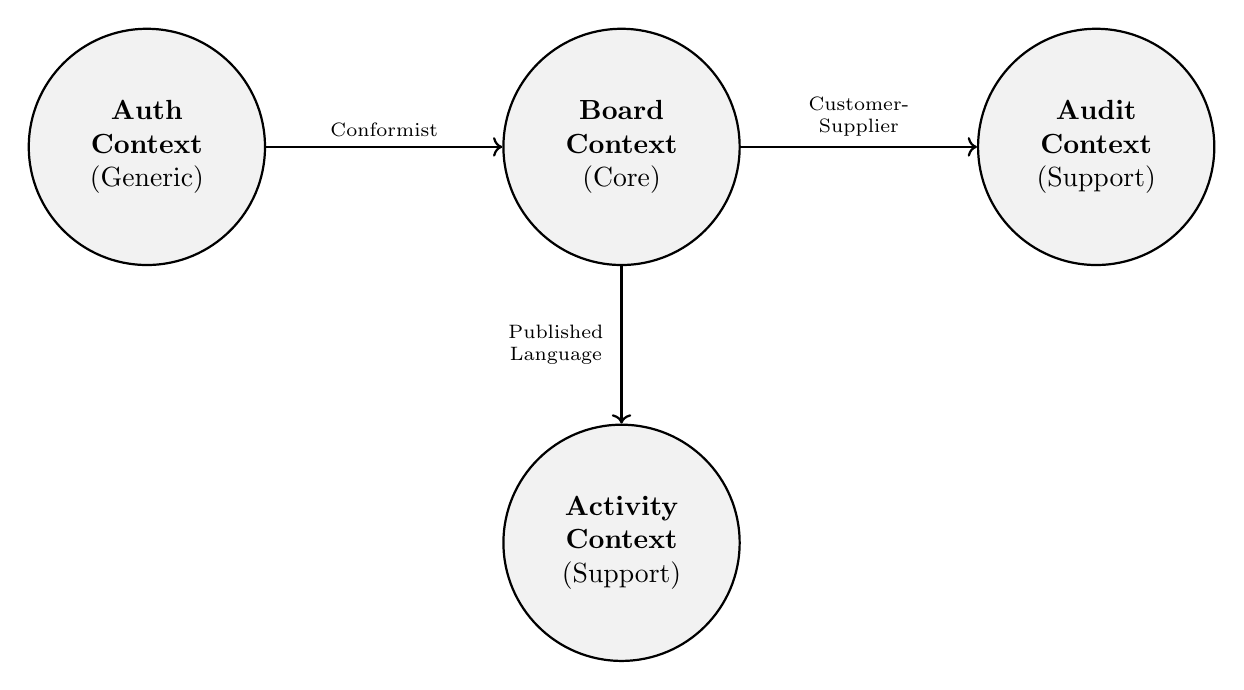
\begin{tikzpicture}[
    node distance=2cm and 3cm,
    context/.style={circle, draw, fill=gray!10, text width=6em, text centered, minimum size=3cm, thick},
    rel/.style={text width=4em, text centered, font=\scriptsize}
]
    \node [context] (board) {\textbf{Board Context} \\ (Core)};
    \node [context, left=of board] (auth) {\textbf{Auth Context} \\ (Generic)};
    \node [context, right=of board] (audit) {\textbf{Audit Context} \\ (Support)};
    \node [context, below=of board] (activity) {\textbf{Activity Context} \\ (Support)};

    % Relationships
    \draw [->, thick] (auth) -- node [above, rel] {Conformist} (board);
    \draw [->, thick] (board) -- node [above, rel] {Customer-Supplier} (audit);
    \draw [->, thick] (board) -- node [left, rel] {Published Language} (activity);

\end{tikzpicture}
}
\caption{Context Map}
\label{fig:context_map}
\end{figure}

\textbf{Relationship Definitions:}
\begin{itemize}
    \item \textbf{Conformist}: The Board Context conforms to the Auth Context's model (user IDs, roles) without negotiation.
    \item \textbf{Customer-Supplier}: The Board Context (Supplier) produces events that the Audit Context (Customer) consumes. The Audit Context relies on the Board Context to provide data in a specific format.
    \item \textbf{Published Language}: The Board Context publishes events (e.g., `TaskMoved`) using a standard schema that the Activity Context subscribes to.
\end{itemize}

\section{Tactical Design}
Tactical design details the technical implementation of the bounded contexts, including the technology stack and internal patterns.

\subsection{Technology Stack}
The project utilizes a modern, performance-oriented stack:
\begin{itemize}
    \item \textbf{Runtime}: \textbf{Bun} (v1.x) for both backend services and frontend tooling.
    \item \textbf{Backend}:
    \begin{itemize}
        \item \textbf{Framework}: \textbf{Hono} for high-performance HTTP APIs.
        \item \textbf{Validation}: \textbf{Zod} for schema validation and type safety.
        \item \textbf{Auth}: \textbf{Better-Auth} for comprehensive authentication.
        \item \textbf{Logging}: \textbf{Pino} for structured logging.
        \item \textbf{Testing}: \textbf{Vitest} for unit and integration tests.
        \item \textbf{Documentation}: \textbf{Scalar} for OpenAPI documentation.
    \end{itemize}
    \item \textbf{Frontend}:
    \begin{itemize}
        \item \textbf{Framework}: \textbf{React} with \textbf{Vite}.
        \item \textbf{Full-Stack Features}: \textbf{TanStack Start} and \textbf{Nitro} server.
        \item \textbf{Routing}: \textbf{TanStack Router}.
        \item \textbf{State Management}: \textbf{TanStack Query}.
        \item \textbf{Styling}: \textbf{TailwindCSS}.
        \item \textbf{UI Components}: \textbf{Lucide-React} (icons), \textbf{DnD-Kit} (drag and drop).
    \end{itemize}
    \item \textbf{Data \& Messaging}:
    \begin{itemize}
        \item \textbf{Database}: \textbf{MongoDB} (Mongoose ORM).
        \item \textbf{Cache}: \textbf{Redis} (IORedis).
        \item \textbf{Messaging}: \textbf{Kafka} (KafkaJS, Strimzi Operator).
    \end{itemize}
\end{itemize}

\subsection{Service Architecture}
Each service is built independently. The following diagram shows the typical internal structure of a service in Cascade.

\begin{figure}[H]
\centering
\resizebox{\textwidth}{!}{
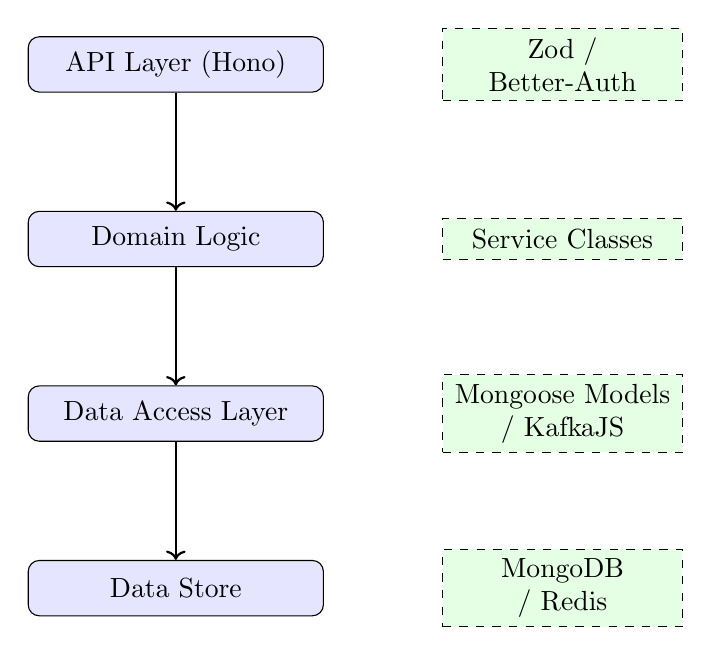
\begin{tikzpicture}[
    node distance=1.5cm,
    auto,
    layer/.style={rectangle, draw, fill=blue!10, text width=10em, text centered, minimum height=2em, rounded corners},
    tech/.style={rectangle, draw, fill=green!10, text width=8em, text centered, minimum height=1.5em, dashed}
]
    \node [layer] (api) {API Layer (Hono)};
    \node [tech, right=of api] {Zod / Better-Auth};
    
    \node [layer, below=of api] (domain) {Domain Logic};
    \node [tech, right=of domain] {Service Classes};
    
    \node [layer, below=of domain] (infra) {Data Access Layer};
    \node [tech, right=of infra] {Mongoose Models / KafkaJS};
    
    \node [layer, below=of infra] (data) {Data Store};
    \node [tech, right=of data] {MongoDB / Redis};

    \draw [->, thick] (api) -- (domain);
    \draw [->, thick] (domain) -- (infra);
    \draw [->, thick] (infra) -- (data);

\end{tikzpicture}
}
\caption{Service Internal Architecture}
\label{fig:service_arch}
\end{figure}

\section{System Architecture}

\subsection{Network Architecture}
The network flow is managed by an Nginx Ingress Controller.

\begin{figure}[H]
\centering
\resizebox{\textwidth}{!}{
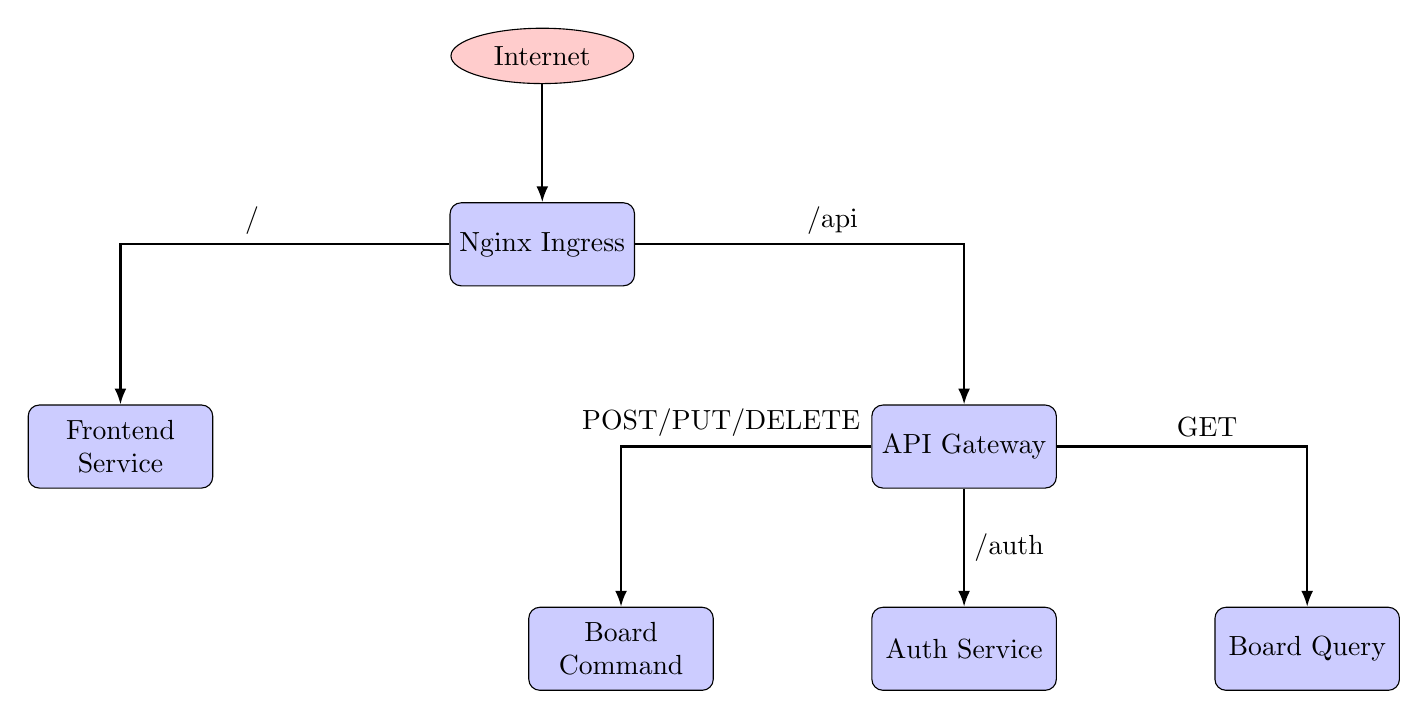
\begin{tikzpicture}[
    node distance=1.5cm and 2cm,
    auto,
    block/.style={rectangle, draw, fill=blue!20, text width=6em, text centered, rounded corners, minimum height=3em},
    cloud/.style={draw, ellipse, fill=red!20, minimum height=2em, text width=4em, text centered},
    line/.style={draw, -{Latex[length=2mm]}, thick}
]
    % Nodes
    \node [cloud] (internet) {Internet};
    \node [block, below=of internet] (ingress) {Nginx Ingress};
    \node [block, below left=of ingress, xshift=-1cm] (frontend) {Frontend Service};
    \node [block, below right=of ingress, xshift=1cm] (gateway) {API Gateway};
    \node [block, below=of gateway] (auth) {Auth Service};
    \node [block, left=of auth] (command) {Board Command};
    \node [block, right=of auth] (query) {Board Query};
    
    % Edges
    \path [line] (internet) -- (ingress);
    \path [line] (ingress) -| node [pos=0.3, above, fill=white] {/} (frontend);
    \path [line] (ingress) -| node [pos=0.3, above, fill=white] {/api} (gateway);
    \path [line] (gateway) -- node [right, fill=white] {/auth} (auth);
    \path [line] (gateway) -| node [pos=0.3, above, fill=white] {POST/PUT/DELETE} (command);
    \path [line] (gateway) -| node [pos=0.3, above, fill=white] {GET} (query);
\end{tikzpicture}
}
\caption{Network Flow Diagram}
\label{fig:network_flow}
\end{figure}

\subsection{Microservices \& CQRS}
The system implements CQRS and Event Sourcing patterns.

\begin{figure}[H]
\centering
\resizebox{\textwidth}{!}{
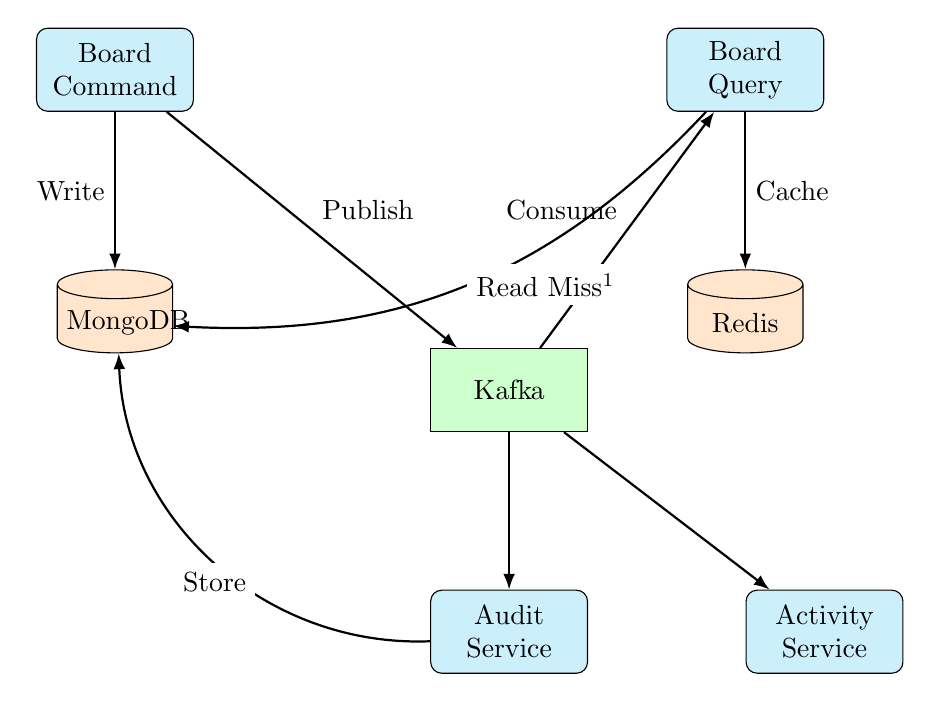
\begin{tikzpicture}[
    node distance=2cm and 2cm,
    auto,
    service/.style={rectangle, draw, fill=cyan!20, text width=5em, text centered, rounded corners, minimum height=3em},
    db/.style={cylinder, draw, shape border rotate=90, fill=orange!20, text width=3.5em, text centered, minimum height=3em, aspect=0.25},
    queue/.style={rectangle, draw, fill=green!20, text width=5em, text centered, minimum height=3em},
    line/.style={draw, -{Latex[length=2mm]}, thick}
]
    \node [service] (command) {Board Command};
    \node [service, right=of command, xshift=4cm] (query) {Board Query};
    \node [queue, below right=of command, xshift=1cm, yshift=-1cm] (kafka) {Kafka};
    \node [db, below=of command] (mongodb) {MongoDB};
    \node [db, below=of query] (redis) {Redis};
    \node [service, below=of kafka] (audit) {Audit Service};
    \node [service, right=of audit] (activity) {Activity Service};
    
    \path [line] (command) -- node [left] {Write} (mongodb);
    \path [line] (command) -- node [above right, fill=white] {Publish} (kafka);
    \path [line] (kafka) -- node [above left, fill=white] {Consume} (query);
    \path [line] (query) -- node [right] {Cache} (redis);
    \path [line] (query) edge [bend left=25] node [right, fill=white] {Read Miss\footnotemark} (mongodb);
    \path [line] (kafka) -- (audit);
    \path [line] (kafka) -- (activity);
    \path [line] (audit) edge [bend left=45] node [below, fill=white] {Store} (mongodb);
\end{tikzpicture}
}
\caption{CQRS and Event-Driven Architecture}
\label{fig:cqrs_arch}
\end{figure}
\footnotetext{Read Miss: If data is not found in Redis, the service queries MongoDB directly.}

\subsection{Event Flow}
\begin{figure}[H]
\centering
\resizebox{\textwidth}{!}{
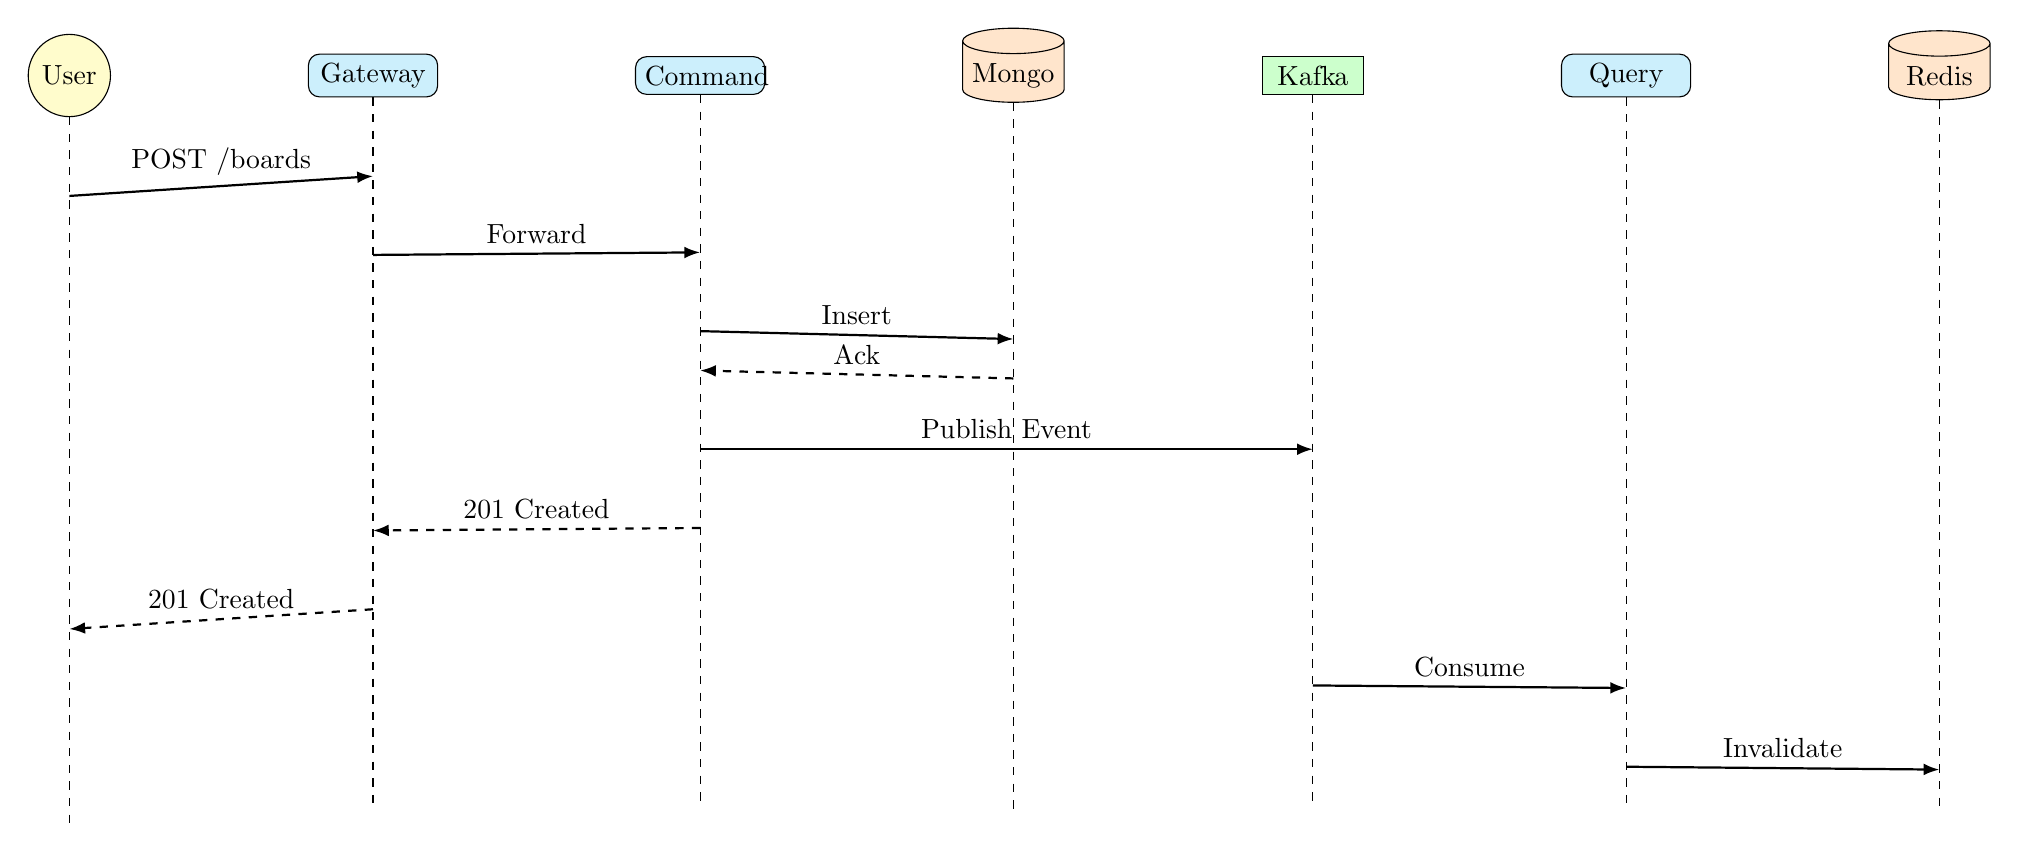
\begin{tikzpicture}[
    node distance=2.5cm,
    auto,
    actor/.style={shape=circle, draw, minimum size=1cm, fill=yellow!20},
    service/.style={rectangle, draw, fill=cyan!20, text width=4em, text centered, rounded corners},
    db/.style={cylinder, draw, shape border rotate=90, fill=orange!20, text width=3em, text centered, aspect=0.25},
    queue/.style={rectangle, draw, fill=green!20, text width=3em, text centered},
    line/.style={draw, -{Latex[length=2mm]}, thick}
]
    \node [actor] (user) {User};
    \node [service, right=of user] (gateway) {Gateway};
    \node [service, right=of gateway] (command) {Command};
    \node [db, right=of command] (mongo) {Mongo};
    \node [queue, right=of mongo] (kafka) {Kafka};
    \node [service, right=of kafka] (query) {Query};
    \node [db, right=of query] (redis) {Redis};

    \foreach \x in {user, gateway, command, mongo, kafka, query, redis} {
        \draw [dashed] (\x.south) -- ++(0,-9);
    }

    \draw [line] ($(user.south) + (0,-1)$) -- node [above] {POST /boards} ($(gateway.south) + (0,-1)$);
    \draw [line] ($(gateway.south) + (0,-2)$) -- node [above] {Forward} ($(command.south) + (0,-2)$);
    \draw [line] ($(command.south) + (0,-3)$) -- node [above] {Insert} ($(mongo.south) + (0,-3)$);
    \draw [line, dashed] ($(mongo.south) + (0,-3.5)$) -- node [above] {Ack} ($(command.south) + (0,-3.5)$);
    \draw [line] ($(command.south) + (0,-4.5)$) -- node [above] {Publish Event} ($(kafka.south) + (0,-4.5)$);
    \draw [line, dashed] ($(command.south) + (0,-5.5)$) -- node [above] {201 Created} ($(gateway.south) + (0,-5.5)$);
    \draw [line, dashed] ($(gateway.south) + (0,-6.5)$) -- node [above] {201 Created} ($(user.south) + (0,-6.5)$);
    \draw [line] ($(kafka.south) + (0,-7.5)$) -- node [above] {Consume} ($(query.south) + (0,-7.5)$);
    \draw [line] ($(query.south) + (0,-8.5)$) -- node [above] {Invalidate} ($(redis.south) + (0,-8.5)$);
\end{tikzpicture}
}
\caption{Board Creation Sequence}
\label{fig:sequence}
\end{figure}

\subsection{Data Model}
\begin{figure}[H]
\centering
\resizebox{\textwidth}{!}{
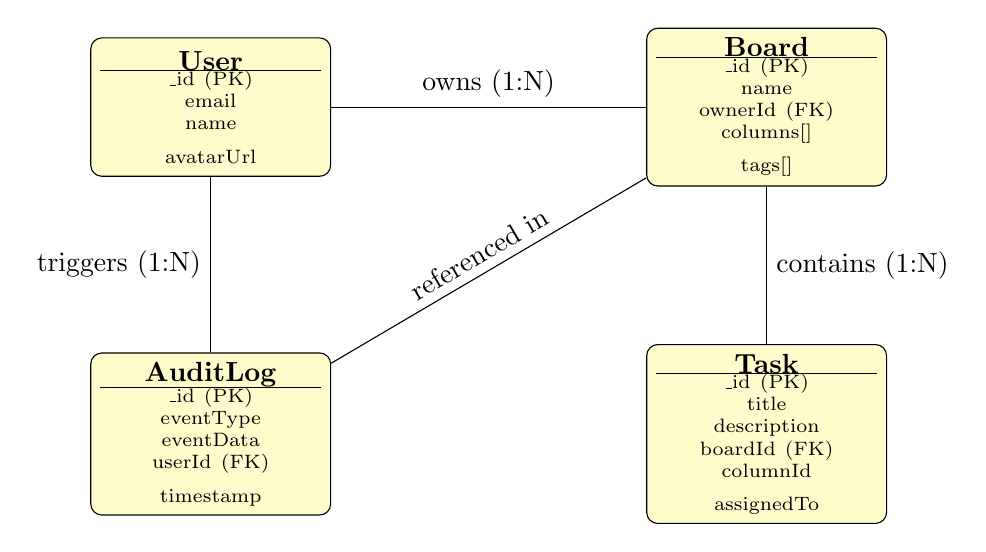
\begin{tikzpicture}[
    node distance=2cm and 4cm,
    entity/.style={rectangle, draw, fill=yellow!20, text width=8em, text centered, minimum height=5em, rounded corners},
    rel/.style={diamond, draw, fill=gray!20, text width=4em, text centered, aspect=2}
]
    \node [entity] (user) {\textbf{User} \\ \hrule \scriptsize \_id (PK) \\ email \\ name \\ avatarUrl};
    \node [entity, right=of user] (board) {\textbf{Board} \\ \hrule \scriptsize \_id (PK) \\ name \\ ownerId (FK) \\ columns[] \\ tags[]};
    \node [entity, below=of board] (task) {\textbf{Task} \\ \hrule \scriptsize \_id (PK) \\ title \\ description \\ boardId (FK) \\ columnId \\ assignedTo};
    \node [entity, left=of task] (audit) {\textbf{AuditLog} \\ \hrule \scriptsize \_id (PK) \\ eventType \\ eventData \\ userId (FK) \\ timestamp};

    \draw (user) -- node [above] {owns (1:N)} (board);
    \draw (board) -- node [right] {contains (1:N)} (task);
    \draw (user) -- node [left] {triggers (1:N)} (audit);
    \draw (board) -- node [above, sloped] {referenced in} (audit);
\end{tikzpicture}
}
\caption{Entity Relationship Diagram}
\label{fig:erd}
\end{figure}

\section{Microservices Patterns}
The architecture implements several key microservices patterns to ensure scalability, resilience, and maintainability.

\subsection{Pattern 1: CQRS (Command Query Responsibility Segregation)}
\begin{itemize}
    \item \textbf{Implementation}: Separate services for write operations (\texttt{board-command}) and read operations (\texttt{board-query}).
    \item \textbf{Benefits}: Allows independent scaling of read and write workloads; optimizes read performance using Redis caching.
\end{itemize}

\subsection{Pattern 2: API Gateway}
\begin{itemize}
    \item \textbf{Implementation}: Nginx acts as the single entry point, routing requests based on path and method.
    \item \textbf{Routing}:
    \begin{itemize}
        \item \texttt{GET /api/boards} $\rightarrow$ \texttt{board-query}
        \item \texttt{POST /api/boards} $\rightarrow$ \texttt{board-command}
    \end{itemize}
    \item \textbf{Benefits}: Simplifies client interaction; provides a centralized place for cross-cutting concerns (though Auth is handled by a separate service).
\end{itemize}

\subsection{Pattern 3: Event Sourcing (Partial)}
\begin{itemize}
    \item \textbf{Implementation}: All state changes are published as immutable events to Kafka. The Audit Service maintains a complete log of these events in the \texttt{cascade-audit} database.
    \item \textbf{Benefits}: Provides a complete audit trail; enables event replay for debugging or rebuilding state.
\end{itemize}

\subsection{Pattern 4: Database per Service}
\begin{itemize}
    \item \textbf{Implementation}: Each service owns its data.
    \begin{itemize}
        \item \texttt{cascade-auth} DB $\rightarrow$ Auth Service
        \item \texttt{cascade-board} DB $\rightarrow$ Board Services (Shared for pragmatic reasons)
        \item \texttt{cascade-audit} DB $\rightarrow$ Audit Service
    \end{itemize}
    \item \textbf{Benefits}: Ensures loose coupling; prevents one service from inadvertently breaking another's data schema.
\end{itemize}

\subsection{Pattern 5: Circuit Breaker (via Retry Logic)}
\begin{itemize}
    \item \textbf{Implementation}: Kafka consumers implement retry logic with exponential backoff for handling message processing failures.
    \item \textbf{Benefits}: Prevents cascading failures; allows the system to recover gracefully from transient errors.
\end{itemize}

\section{Key Architectural Decisions}
\begin{enumerate}
    \item \textbf{Pragmatic CQRS}: Both Command and Query services share the same MongoDB physical cluster but use different logical databases/collections where appropriate. This reduces infrastructure cost while maintaining logical separation.
    \item \textbf{Eventual Consistency}: The system accepts a small window of inconsistency (typically $<$500ms) between a write (Command) and a read (Query) to achieve high performance.
    \item \textbf{Stateless Services}: All application services are stateless, allowing for easy horizontal scaling via Kubernetes Deployments.
    \item \textbf{Infrastructure as Code}: The entire deployment is managed via Helm charts, ensuring reproducibility.
\end{enumerate}

\section{Kubernetes Infrastructure}
The application is deployed on GKE with a robust configuration of resources.

\subsection{Workloads}
The system consists of 8 deployed microservices:
\begin{itemize}
    \item \textbf{Deployments}:
    \begin{itemize}
        \item \texttt{cascade-frontend} (Port 3000): Serves the React application.
        \item \texttt{cascade-api-gateway} (Nginx): Reverse proxy and routing.
        \item \texttt{cascade-auth} (Port 3001): Authentication service.
        \item \texttt{cascade-board-command} (Port 3002): Write operations.
        \item \texttt{cascade-board-query} (Port 3003): Read operations.
        \item \texttt{cascade-activity} (Port 3004): Activity tracking.
        \item \texttt{cascade-audit} (Port 3005): Audit logging.
        \item \texttt{cascade-api-docs} (Port 3006): Scalar documentation.
    \end{itemize}
    \item \textbf{StatefulSets}:
    \begin{itemize}
        \item \texttt{cascade-mongodb}: A 3-node replica set. StatefulSets are used here to maintain stable network identities (\texttt{cascade-mongodb-0}, etc.) and persistent storage for data safety.
    \end{itemize}
    \item \textbf{Jobs}:
    \begin{itemize}
        \item \texttt{cascade-mongodb-init}: A one-time job that connects to the MongoDB pods and initiates the replica set configuration.
    \end{itemize}
\end{itemize}

\subsection{Services and Networking}
\begin{itemize}
    \item \textbf{ClusterIP}: The default service type. Used for internal communication (e.g., \texttt{cascade-auth}, \texttt{cascade-redis-master}). These are not exposed externally.
    \item \textbf{Headless Services}: Used for MongoDB (\texttt{cascade-mongodb-headless}) and Kafka to allow direct pod discovery and stable DNS entries for clustering.
    \item \textbf{Ingress}: The single entry point for external traffic, routing to the API Gateway and Frontend based on path rules.
\end{itemize}

\subsection{Autoscaling (HPA)}
Horizontal Pod Autoscalers are configured for critical services to handle varying loads:
\begin{itemize}
    \item \texttt{cascade-auth}, \texttt{cascade-board-command}, \texttt{cascade-board-query}, \texttt{cascade-frontend}.
    \item \textbf{Policy}: Scale between 1 and 5 replicas based on CPU utilization (target 80\%).
\end{itemize}

\subsection{Event Streaming Infrastructure}
\begin{itemize}
    \item \textbf{Strimzi Operator}: Manages the Kafka cluster.
    \item \textbf{Kafka Cluster}: Running in KRaft mode (no Zookeeper).
    \item \textbf{Kafka UI}: Deployed for easy monitoring and management of topics and messages.
\end{itemize}

\chapter{Services}

\section{Auth Service}
The Auth Service handles user authentication and session management.
\begin{itemize}
    \item \textbf{Port}: 3001
    \item \textbf{Database}: \texttt{cascade-auth}
    \item \textbf{Features}:
    \begin{itemize}
        \item Email/Password authentication via Better Auth.
        \item GitHub OAuth integration.
        \item JWT token generation and validation.
    \end{itemize}
\end{itemize}

\section{Board Command Service}
Responsible for all write operations to boards and tasks.
\begin{itemize}
    \item \textbf{Port}: 3002
    \item \textbf{Database}: \texttt{cascade-board}
    \item \textbf{Responsibilities}:
    \begin{itemize}
        \item Validating incoming requests (Zod schemas).
        \item Persisting changes to MongoDB.
        \item Publishing domain events to Kafka (e.g., \texttt{board.created}, \texttt{task.moved}).
    \end{itemize}
\end{itemize}

\section{Board Query Service}
Responsible for serving read requests with high performance.
\begin{itemize}
    \item \textbf{Port}: 3003
    \item \textbf{Database}: \texttt{cascade-board}
    \item \textbf{Cache}: Redis
    \item \textbf{Responsibilities}:
    \begin{itemize}
        \item Serving GET requests for boards and tasks.
        \item Managing Redis cache (Read-through/Write-through).
        \item Consuming Kafka events to invalidate stale cache entries.
    \end{itemize}
\end{itemize}

\section{Activity Service}
Provides real-time visibility into system activities.
\begin{itemize}
    \item \textbf{Port}: 3004
    \item \textbf{Input}: Kafka topics
    \item \textbf{Function}: Consumes events and logs them for monitoring. It does not maintain its own database but streams activity data.
\end{itemize}

\section{Audit Service}
Ensures compliance and security through immutable logging.
\begin{itemize}
    \item \textbf{Port}: 3005
    \item \textbf{Database}: \texttt{cascade-audit}
    \item \textbf{Function}: Consumes all domain events and stores them in an append-only collection.
    \item \textbf{Schema}: Includes \texttt{eventType}, \texttt{eventData}, \texttt{userId}, and \texttt{timestamp}.
\end{itemize}

\section{API Docs Service}
Hosts the interactive API documentation.
\begin{itemize}
    \item \textbf{Port}: 3006
    \item \textbf{Tool}: Scalar
    \item \textbf{Path}: \texttt{/reference}
\end{itemize}

\chapter{Deployment}

\section{Prerequisites}
Before deploying Cascade, ensure you have the following tools installed:
\begin{itemize}
    \item Docker and Docker Compose
    \item Google Cloud SDK (gcloud)
    \item kubectl
    \item Helm
\end{itemize}

\section{Local Development}
For local development, Docker Compose is used to spin up the entire stack.
\begin{lstlisting}[language=bash, caption=Start Local Environment]
docker-compose up --build
\end{lstlisting}
This starts all microservices, MongoDB, Redis, and Kafka locally.

\section{GKE Deployment}
Deploying to Google Kubernetes Engine involves several steps, automated via Helm and shell scripts.

\subsection{Setup Script}
The \texttt{setup.sh} script automates the cluster creation and configuration.
\begin{lstlisting}[language=bash, caption=Run Setup Script]
./setup.sh <YOUR_PROJECT_ID>
\end{lstlisting}

\subsection{Helm Charts}
The project uses a unified Helm chart located in \texttt{helm/cascade}.
Key configuration files:
\begin{itemize}
    \item \texttt{values.yaml}: Default configuration values.
    \item \texttt{templates/}: Kubernetes manifest templates.
\end{itemize}

\subsection{Manual Deployment Steps}
If not using the setup script:
\begin{enumerate}
    \item \textbf{Create Cluster}: Create a GKE cluster with standard settings.
    \item \textbf{Install Dependencies}: Install Nginx Ingress Controller and Cert Manager (if needed).
    \item \textbf{Build Images}: Build and push Docker images to Google Artifact Registry.
    \item \textbf{Deploy Helm Chart}:
    \begin{lstlisting}[language=bash]
    helm install cascade ./helm/cascade --set project.id=<PROJECT_ID>
    \end{lstlisting}
\end{enumerate}

\section{Configuration}
\subsection{Environment Variables}
Services are configured via environment variables injected by Kubernetes.
\begin{itemize}
    \item \texttt{MONGODB\_URI}: Connection string for MongoDB.
    \item \texttt{KAFKA\_BROKERS}: Address of Kafka bootstrap server.
    \item \texttt{REDIS\_HOST}: Address of Redis instance.
    \item \texttt{JWT\_SECRET}: Secret key for signing tokens.
\end{itemize}

\subsection{Secrets Management}
Sensitive data like OAuth secrets and database credentials should be managed using Kubernetes Secrets, not plain text in \texttt{values.yaml}.

\chapter{API Reference}

\section{Overview}
The API is designed around RESTful principles. All API endpoints are prefixed with \texttt{/api}.

\section{Authentication Endpoints}
\begin{itemize}
    \item \texttt{POST /api/auth/sign-up}: Register a new user.
    \item \texttt{POST /api/auth/sign-in}: Log in an existing user.
    \item \texttt{POST /api/auth/sign-out}: Log out.
    \item \texttt{GET /api/auth/session}: Get current session.
\end{itemize}

\section{Board Endpoints}
\begin{itemize}
    \item \texttt{GET /api/boards}: List all boards for the current user.
    \item \texttt{POST /api/boards}: Create a new board.
    \item \texttt{GET /api/boards/:id}: Get details of a specific board.
    \item \texttt{PUT /api/boards/:id}: Update a board.
    \item \texttt{DELETE /api/boards/:id}: Delete a board.
\end{itemize}

\section{Task Endpoints}
\begin{itemize}
    \item \texttt{POST /api/tasks}: Create a new task.
    \item \texttt{PUT /api/tasks/:id}: Update a task (move, edit).
    \item \texttt{DELETE /api/tasks/:id}: Delete a task.
\end{itemize}

\section{Interactive Documentation}
For interactive testing and detailed schema information, visit the API Docs service at \texttt{/reference} when the application is running.


\end{document}
